\section{Бројна вредност логаритма}\index{бројна вредност}

\subsection{Формула}

Бројна вредност природног логаритма може бити израчуната помоћу формуле
\begin{equation}\index{формула}\index{ln@$\ln$}
\okvir{
\ln x
%&=2\mathop{\rm arctanh}\frac{x-1}{x+1}\\
=\sum_{n=0}^\infty\frac{2}{2n+1}\left(\frac{x-1}{x+1}\right)^{\!2n+1}
}
\label{eq:lnred}
\end{equation}
до жељене тачности.
Поступак којим се рачуна $y=\ln x$ са тачношћу $\varepsilon$\index{епсилон $(\varepsilon)$}
изгледа овако:
\def\asg{\leftarrow}%
\begin{equation}\index{алгоритам}
\label{eq:alg}
\begingroup\color{Blue}
\ram{\enspace
\begin{aligned}
&r\asg(x-1)/(x+1);\quad k\asg 1;\quad p\asg 2r;\quad q\asg r^2;\quad a\asg p;\quad y\asg a;\\
&\text{понављати док је $|a|>\varepsilon$:}\\
&\qquad k\asg k+2;\quad p\asg p\cdot q;\quad a\asg p/k;\quad y\asg y+a;
\end{aligned}
\enspace}
\endgroup
\end{equation}
Овим поступком се може израчунати вредност
\begin{align}
  \begin{split}\label{eq:ln2}\index{ln2@$\ln 2$}
    \ln2
    & = \frac{2}{1\cdot3^1}+\frac{2}{3\cdot3^3}+\frac{2}{5\cdot3^5}+\frac{2}{7\cdot3^7}+\frac{2}{9\cdot3^9}+\cdots\\
    \noalign{\smallskip}
    & = 0\.
    6931471805\,
    5994530941\,
    7232121458\,
    1765680755\,
    \ldots
  \end{split}
  \intertext{као и вредност}
  \begin{split}\label{eq:ln10}\index{ln10@$\ln10$}
    \ln10
    & = \frac{2}{1\cdot9^1}+\frac{2}{3\cdot9^3}+\frac{2}{5\cdot9^5}+\frac{2}{7\cdot9^7}+\frac{2}{9\cdot9^9}+\cdots+3\ln2\\
    \noalign{\smallskip}
    & = 2\.
    3025850929\,
    9404568401\,
    7991454684\,
    3642076011\,
    \ldots
  \end{split}
\end{align}
(Видети задатак \ref{sssec:ln3} на страни \pageref{sssec:ln3}.)
Помоћу њих се могу израчунати бројне вредности бинарног
$\logtwo x=\ln x/\ln2$, односно, декадног
$\logten x=\ln x/\ln 10$ логаритма.

\subsection{Верижни разломак}\index{верижни разломак}

Бројна вредност природног логаритма може бити израчуната и помоћу {\sl верижног разломка}
\begin{equation}\label{eq:verige}
\begin{aligned}
\noalign{\vskip-6pt}
\ln(1+x)
&=\cfrac{x}{1+\cfrac{1^2x}{2-1x+\cfrac{2^2x}{3-2x+\cfrac{3^2x}{4-3x+\ddots}}}}\\
\noalign{\vskip-6pt}
&=\cfrac{x}{1+ \Kinf{\n^2x}{\n+1-\n x}}.
\end{aligned}
\end{equation}
Попут симбола које се користе за суму `$\rm\Sigma$' или производ `$\rm\Pi$', 
\idx{Гаус} (Johann Carl Friedrich Gau\ss) је смислио погодан начин за представљање
верижних ({\sl ланчаних\/}) разломака,
где симбол `K' потиче од немачке речи за {\sl прекинути ланац\/} ({\sl Kettenbruch\/}).
Израз иза овог симбола показује како изгледа {\sl општи члан\/} верижног разломка.

\def\ff#1/#2,{\frac{#1}{#2},}
Ако помоћу ове формуле израчунамо првих 11 {\sl конвергената\/}\index{конвергент} $\ln2$ као $-\ln(1+x)$, 
где је $x=-1/2$,
добићемо
$$
\ln2\approx\ff1/2, \ff5/8, \ff2/3, \ff131/192, \ff661/960, \ff1327/1920, \ff1163/1680, \ff148969/215040, 
\ff447047/645120, \ff44711/64512, \ff983705/1419264, \dots
$$
где је последњи разломак тачан на 5 децимала.


\subsection{Логаритамске таблице}\index{таблице}

Прве таблице логаритама је 1614.\ године 
израчунао шкотски математичар \idx{Непер} (John Napier of Merchiston),
које су садржале логаритме за основу $(1-1/10^7)^{10^7} \approx1/\e$, 
са скалираним аргументом и резултатом,
иако сам Непер није знао за константу $\e$.
Савременим записом би логаритам из Неперових таблица био дефинисан као
$$
\naplog (x) = \log_{1-1/10^7}(x/10^7)
\approx 10^7\log_{1/\e}(x/10^7) = -10^7\ln(x/10^7).
$$

Неколико година касније, 1617.\ и 1624,\ 
енглески математичар \idx{Бригс} (Henry Briggs) је израчунао
таблице декадних логаритама са 14 цифара тачности, које се уз допуне и исправке
користе и данас под именом {\sl Бригсове таблице}.


\subsection{Логаритмар}\index{логаритмар}

\input siber

Пре појаве дигитрона\index{дигитрон}, за приближно одређивање бројне вредности логаритма,
користила се је аналогна механичка справа са неколико лењира звана
{\sl логаритмар}\index{шибер}.
$$
\slika{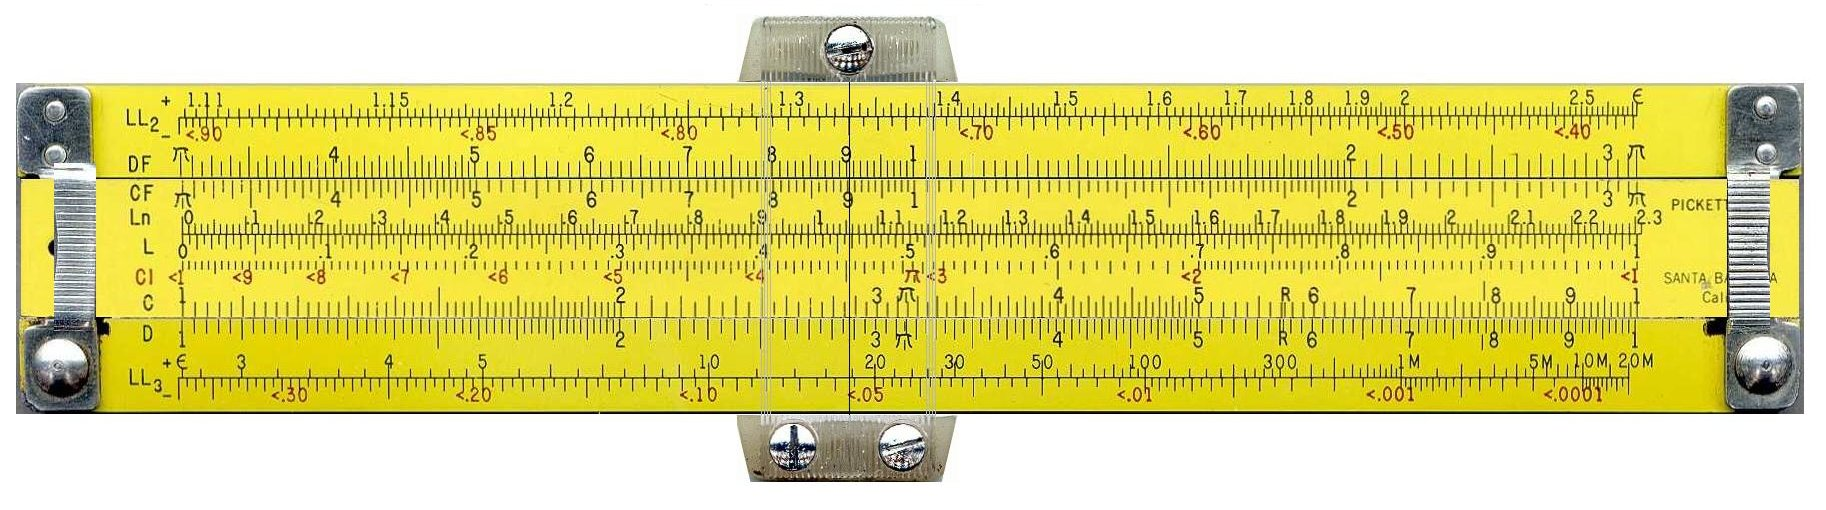
\includegraphics[width=0.90\textwidth]{siber2.jpg}}{Шибер.}
$$
Лењири имају подеоке са децималном и логаритамском, а често и са синусном и неком другом скалом.
Један од лењира је {\sl клизни}, те отуда популарно име \hbox{\sl шибер\/}
(од немачког {\sl Rechen\-schieber\/}). 
Користи се једноставно, померањем клизача и читањем вредности са одговарајуће скале.
(Видети задатке~\ref{sssec:siberpower} и~\ref{sssec:sibersqrt}.)

Постојале су и кружне варијанте,
%  (види страну \pageref{circlog})
па и џепне, где је
џепни сат са логаритмаром и компасом био
\navod{\idx{iPhone}} XIX и прве половине XX~века.
$$
\slika{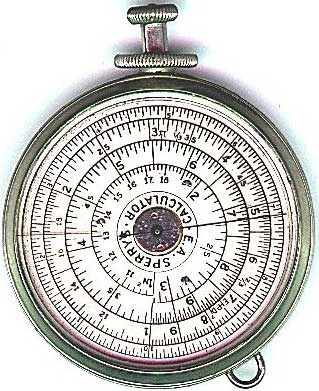
\includegraphics[width=50\mm]{sahat.jpg}}{Џепни логаритмар.}
$$

Таблице и логаритмари се и данас користе у војсци, као резерва у случају отка\-зи\-вања електронике.
Први \idx{компјутер} ENIAC\index{ениац@ENIAC} (Electronic Numerical Integrator And Computer)
је направљен 1946.\ године са наменом да израчуна таблице за војску.
